\section{Position and Orientation}
\subsection{Introduction}
Kinematics studies the movement of an object -- in our case of a robot -- without taking into acount the forces generating it. Instead, it only handles aspects such as position, orientation, speed and momentum of bodies in movement.

Consider for instance a robotic arm. We can design a simplified scheme of the robot and its environment, to create a kinematic pipeline and reference frames associated to each of these objects.

\begin{figure}[H]
    \centering
    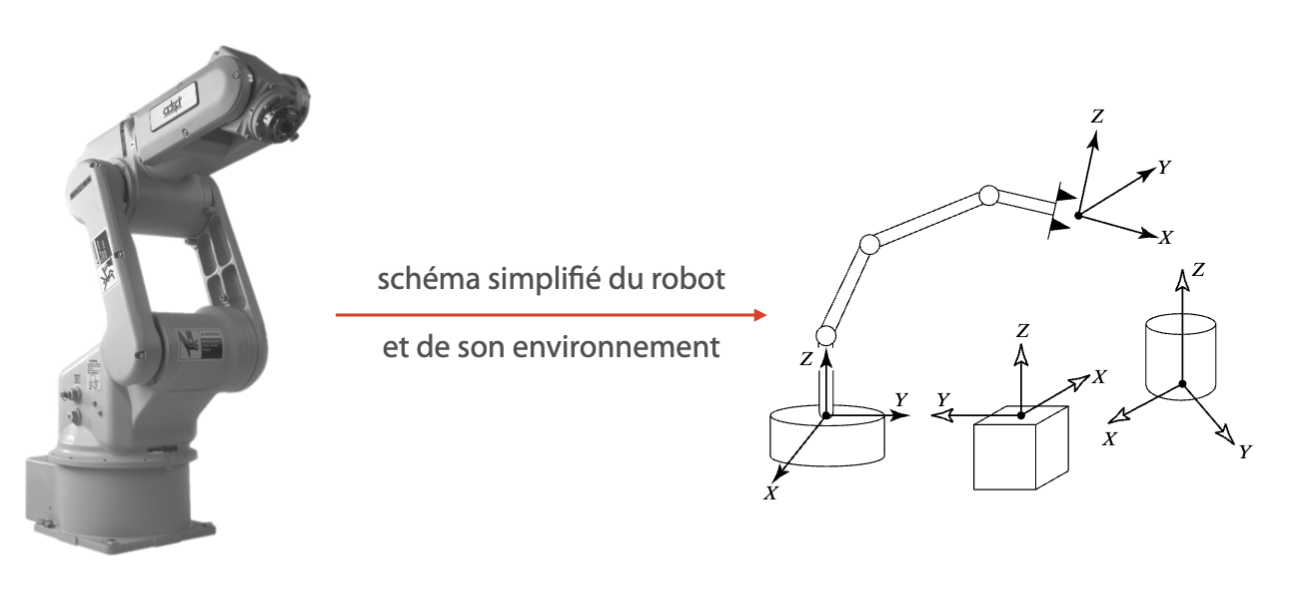
\includegraphics[width=.6\textwidth]{position/arm-scheme.png}
    \caption{Simplified scheme of the robot feature the kinematic pipeline and reference frames.}
\end{figure}

\emph{Direct kinematics} allows to compute the position and orientation of the terminal organ given, for instance, the angles of the articulations.

\begin{figure}[H]
    \centering
    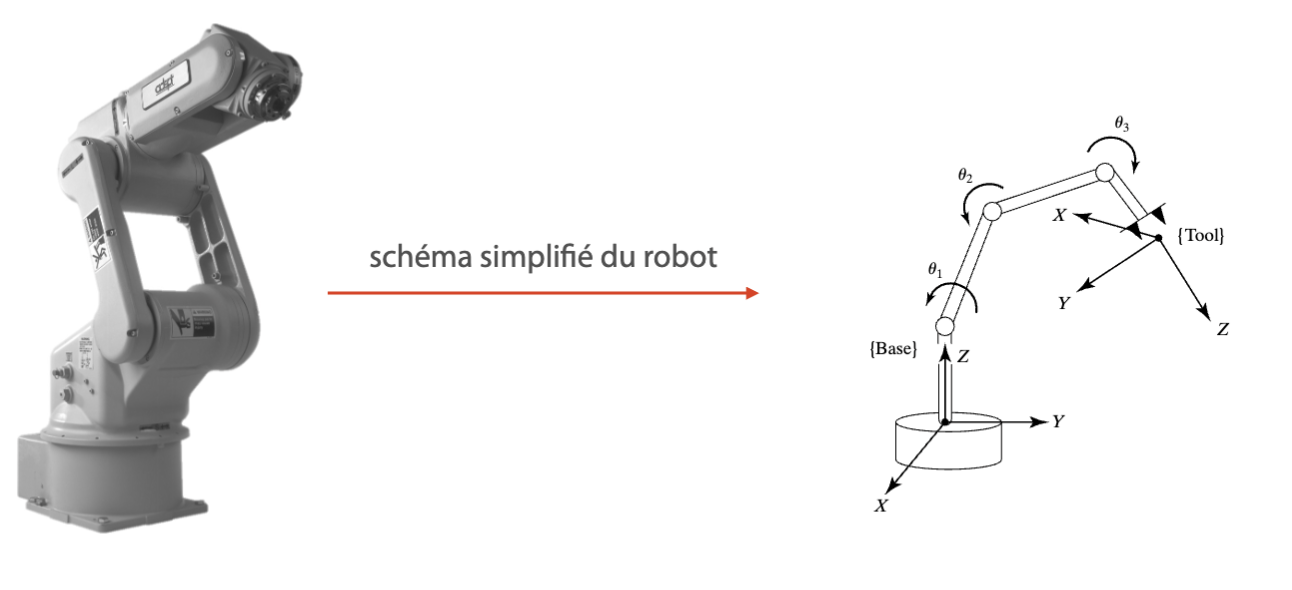
\includegraphics[width=.6\textwidth]{position/direct-kinematic.png}
\end{figure}

\emph{Invert kinematics} answers the question the other way around: given the position and orientation of a boyd, how can we compute the values of the articulations angles. Invert kinematics is used for instance for trajectory tracking: given a reference trajectory, how can we compute the speed of the articulations?

\subsection{Points, frames and transformations}
\subsubsection{Position of a point in space}
Once that a reference frame $\{A\}$ is defined, we can localize any point of the universe given a \emph{position vector}:
\begin{figure}[H]
    \centering

    \begin{minipage}{0.4\textwidth}
        \begin{equation*}
            \prescript{A}{}{P} = \begin{bmatrix}
                p_x \\ p_y \\ p_z
            \end{bmatrix}
        \end{equation*}
    \end{minipage}
    \begin{minipage}{0.4\textwidth}
        \centering
        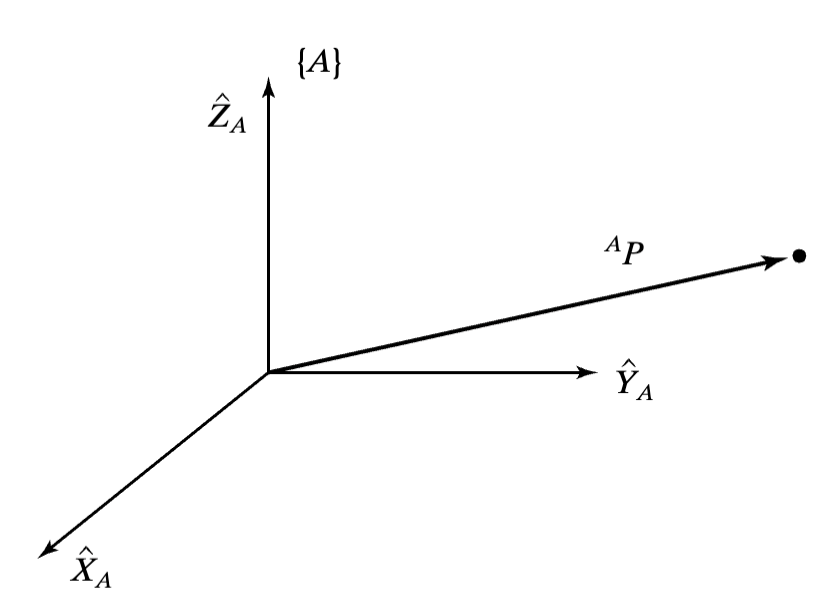
\includegraphics[width=.8\textwidth]{position/position-frame.png}
    \end{minipage}
    \caption{Vector and position of the point established in the frame $\{A\}$.}
\end{figure}

\subsubsection{Position and orientation of a body in space}
To define the orientation of a body in space, we need to define a reference frame $\{B\}$ attached to this body. The orientation is therefore defined as the expression of this coordinate system in the reference frame $\{A\}$.
\begin{figure}[H]
    \centering

    \begin{minipage}{0.5\textwidth}
        \begin{equation*}
            \prescript{A}{B}{R} = \begin{bmatrix}
                \prescript{A}{}{\hat{X}}_B & \prescript{A}{}{\hat{Y}}_B & \prescript{A}{}{\hat{Z}}_B
            \end{bmatrix}
            = \begin{bmatrix}
                r_{11} & r_{12} & r_{13} \\
                r_{21} & r_{22} & r_{23} \\
                r_{31} & r_{32} & r_{33}
            \end{bmatrix}
        \end{equation*}
    \end{minipage}
    \begin{minipage}{0.4\textwidth}
        \centering
        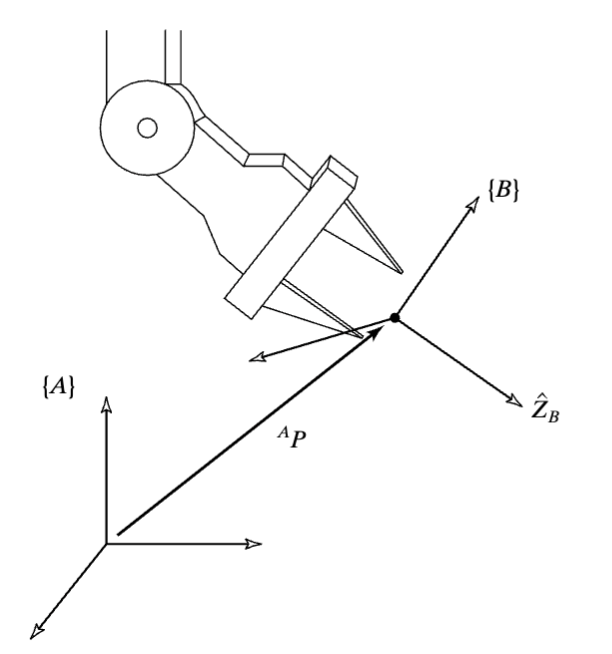
\includegraphics[width=.8\textwidth]{position/body-orientation.png}
    \end{minipage}
    \caption{Expression of the coordinate system $\{B\}$ in the reference frame $\{A\}$, and the associated position and orientation of the body.}
\end{figure}
Each element of the matrix $\prescript{A}{B}{R}$ is the scalar product between the vectors of the two coordinate systems $\{B\}$ and $\{A\}$:
\begin{equation*}
    \prescript{A}{B}{R} = \begin{bmatrix}
        \prescript{A}{}{\hat{X}}_B & \prescript{A}{}{\hat{Y}}_B & \prescript{A}{}{\hat{Z}}_B
    \end{bmatrix}
    = \begin{bmatrix}
        \hat{X}_B\cdot\hat{X}_A & \hat{Y}_B\cdot\hat{X}_A & \hat{Z}_B\cdot\hat{X}_A \\
        \hat{X}_B\cdot\hat{Y}_A & \hat{Y}_B\cdot\hat{Y}_A & \hat{Z}_B\cdot\hat{Y}_A \\
        \hat{X}_B\cdot\hat{Z}_A & \hat{Y}_B\cdot\hat{Z}_A & \hat{Z}_B\cdot\hat{Z}_A
    \end{bmatrix}
\end{equation*}
The lines correspond to the axes of the frame $\{A\}$ expressed in the frame $\{B\}$. Note that the invert of a rotation matrix is its transpose:
\begin{equation*}
    \prescript{A}{B}{R}^T = \prescript{A}{B}{R}^{-1} = \prescript{B}{A}{R}
\end{equation*}

\subsubsection{Rotation matrices}
We showed that the orientation of the body in space could be expressed as a 3-dimensional rotation matrix. The group of 3-dimensional rotation matrices is denoted $\SO(3)$, and is composed of all the matrices that are orthonormal, that is orthogonal and with a determinant equal to 1:
\begin{equation}
    \SO(3) = \set{R\in\mathcal{M}_{3}(\R)}{RR^T=I_3 \text{ and } \det(R) = +1}
\end{equation}
If we write:
\begin{equation*}
    R = \begin{bmatrix}
        \hat{X} & \hat{Y} & \hat{Z}
    \end{bmatrix}
\end{equation*}
Then $R\in\SO(3)$ if and only if:
\begin{equation*}
    \begin{cases}
        \hat{X}\cdot\hat{Y} = 0 \\
        \hat{Y}\cdot\hat{Z} = 0 \\
        \hat{Z}\cdot\hat{X} = 0 \\
    \end{cases}
    \quad\text{and}\quad
    \begin{cases}
        \hat{X}\cdot\hat{X} = 1 \\
        \hat{Y}\cdot\hat{Y} = 1 \\
        \hat{Z}\cdot\hat{Z} = 1 \\
    \end{cases}
\end{equation*}
Note that we have 9 degrees of freedom and 6 independent constraints, so the group $\SO(3)$ is 3-dimensional.

\subsection{Rotation representations}
There are several ways to represent a rotation matrix, each with its own advantages and drawbacks. The most common representations are:
\begin{itemize}
    \item Orthonormal 3 by 3 matrices --- 9 components
    \item Euler angles --- 3 components
    \item Axis-angle representation --- 3 components
    \item Quaternions --- 4 components
\end{itemize}
The number of components used to be an important factor when computers were slow and memory was expensive. Nowadays, the choice of representation is more about the ease of use and the properties of the representation.

\subsubsection{Euler angles}
Each rotation can be represented by the composition of three elementary rotations around the fixed axes of the frame $\{A\}$.
\begin{figure}[H]
    \centering
    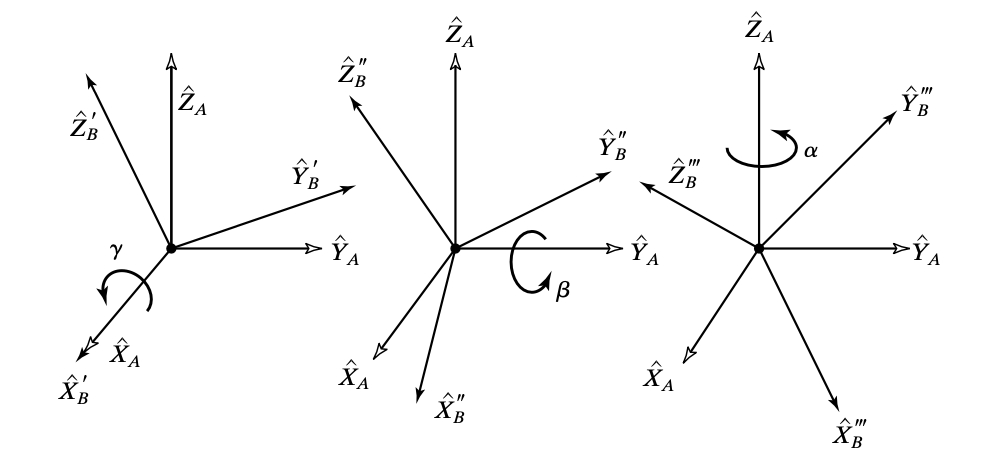
\includegraphics[width=.6\textwidth]{position/euler-angles.png}
    \caption{Euler angles representation of a rotation.}
\end{figure}
In terms of rotation matrices, any rotation matrix can be written as $\prescript{A}{B}{R}(\gamma, \beta, \alpha)$, defined by:
\begin{align*}
    \prescript{A}{B}{R}(\gamma, \beta, \alpha) &= R_Z(\alpha)R_Y(\beta)R_X(\gamma)\\
    &= \begin{bmatrix}
        \cos\alpha & -\sin\alpha & 0 \\
        \sin\alpha & \cos\alpha & 0 \\
        0 & 0 & 1
    \end{bmatrix}
    \begin{bmatrix}
        \cos\beta & 0 & \sin\beta \\
        0 & 1 & 0 \\
        -\sin\beta & 0 & \cos\beta
    \end{bmatrix}
    \begin{bmatrix}
        1 & 0 & 0 \\
        0 & \cos\gamma & -\sin\gamma \\
        0 & \sin\gamma & \cos\gamma
    \end{bmatrix}
\end{align*}
The Euler angles are not unique, as the same rotation can be represented by different sets of Euler angles. This is called gimbal lock, and is a major drawback of the Euler angles representation.

We can also express the Euler angles given the rotation matrix:
\begin{align*}
    \prescript{A}{B}{R}(\gamma, \beta, \alpha) = \begin{bmatrix}
        r_{11} & r_{12} & r_{13} \\
        r_{21} & r_{22} & r_{23} \\
        r_{31} & r_{32} & r_{33}
    \end{bmatrix}
    \implies
    \begin{cases}
        \beta = \atantwo(-r_{31}, \sqrt{r_{11}^2+r_{21}^2}) \\
        \alpha = \atantwo(r_{21}/\cos\beta, r_{11}/\cos\beta) \\
        \gamma = \atantwo(r_{32}/\cos\beta, r_{33}/\cos\beta)
    \end{cases}
\end{align*}

\subsubsection{Axis-angle and quaternions}
We are given a vector $\vec{k}$ and an angle $\theta$; the rotation represented by these two elements is the rotation of angle $\theta$ around the axis $\vec{k}$. We can define:
\begin{equation*}
    \begin{cases}
        \epsilon_1 = k_x\sin\frac{\theta}{2} \\
        \epsilon_2 = k_y\sin\frac{\theta}{2} \\
        \epsilon_3 = k_z\sin\frac{\theta}{2} \\
        \epsilon_4 = \cos\frac{\theta}{2}
    \end{cases}
\end{equation*}
we have $\epsilon_1^2+\epsilon_2^2+\epsilon_3^2+\epsilon_4^2=1$, creating a unit quaternion. The rotation matrix associated to the quaternion is:
\begin{equation*}
    R_\epsilon = \begin{bmatrix}
        1-2\epsilon_2^2-2\epsilon_3^2 & 2(\epsilon_1\epsilon_2-\epsilon_3\epsilon_4) & 2(\epsilon_1\epsilon_3+\epsilon_2\epsilon_4) \\
        2(\epsilon_1\epsilon_2+\epsilon_3\epsilon_4) & 1-2\epsilon_1^2-2\epsilon_3^2 & 2(\epsilon_2\epsilon_3-\epsilon_1\epsilon_4) \\
        2(\epsilon_1\epsilon_3-\epsilon_2\epsilon_4) & 2(\epsilon_2\epsilon_3+\epsilon_1\epsilon_4) & 1-2\epsilon_1^2-2\epsilon_2^2
    \end{bmatrix}
\end{equation*}

The invert operation is also simple to compute:
\begin{align*}
    \prescript{A}{B}{R}(\gamma, \beta, \alpha) = \begin{bmatrix}
        r_{11} & r_{12} & r_{13} \\
        r_{21} & r_{22} & r_{23} \\
        r_{31} & r_{32} & r_{33}
    \end{bmatrix}
    \implies
    \begin{cases}
        \epsilon_1 = \frac{r_{32}-r_{23}}{4\epsilon_4} \\
        \epsilon_2 = \frac{r_{13}-r_{31}}{4\epsilon_4} \\
        \epsilon_3 = \frac{r_{21}-r_{12}}{4\epsilon_4} \\
        \epsilon_4 = \frac{1}{2}\sqrt{1+r_{11}+r_{22}+r_{33}}
    \end{cases}
\end{align*}

\subsection{Angular velocity}
The angular velocity of a body is a vector that describes the rotation of the body in space. It is defined as the derivative of the rotation matrix with respect to time. Angular velocity matrices are skew-symmetric matrices, i.e. matrices of the tangent space of $\SO(3)$, denoted $\so(3)$:
\begin{equation*}
    \so(3) = \set{W\in\mathcal{M}_3(\R)}{W^\tp=-W} = \set{\begin{bmatrix}
        0 & -w_z & w_y \\
        w_z & 0 & -w_x \\
        -w_y & w_x & 0
    \end{bmatrix}}{w_x, w_y, w_z\in\R}
\end{equation*}
Indeed, consider the rotation matrix $R(t)\in\SO(3)$, and denote $\dot R(t) = \partfrac{R(t)}{t}$ the derivative of $R(t)$ with respect to time. We have:
\begin{align*}
    R(t)R(t)^\tp &= I_3 \\
    \dot RR^\tp + R\dot R^\tp &= 0_3 \\
    \dot RR^\tp &= -R\dot R^\tp \\
    \dot RR^\tp &= -\left(\dot RR^\tp\right)^\tp \\
\end{align*}
Hence, by defining $W := \dot RR^\tp$, we have $W\in\so(3)$.

Note that $R(t)$ is the solution of the differential equation $\dot R = WR$, with $R(0)=R_0\in\SO(3)$. The solution is:
\begin{equation*}
    R(t) = R_0\exp(Wt) \quad\text{where}\quad \exp(Wt) = \sum_{n=0}^{+\infty}\frac{(Wt)^n}{n!}
\end{equation*}
This gives us a new parameterization of the group $\SO(3)$, using the angular velocity matrices. Recall that a matrix $W\in\so(3)$ is associated to a vector $w=(w_x, w_y, w_z)\in\R^3$; we denote $\hat{w}=W$. The main question associated to this representation is to compute the infinite sum of the exponential function:
\begin{equation}
    \exp(tW)=\sum_{n=0}^{+\infty}\frac{(tW)^n}{n!}
\end{equation}
We can use the fact that any skew-symmetric matrix $W\in\so(3)$ is nilpotent, i.e. there exists an integer $n\in\N$ such that $W^n=0_3$. This allows us to compute the exponential function:
\begin{equation*}
    \hat{w}=W=\begin{bmatrix}
        0 & -w_z & w_y \\
        w_z & 0 & -w_x \\
        -w_y & w_x & 0
    \end{bmatrix} = w \times \cdot
\end{equation*}
Therefore, $\hat{w}^2=ww^\tp-I_3$, and $\hat{w}^3=-\hat{w}$. We can then regroup the different terms of the exponential function, by transforming the exponents greater than 3:
% TODO: detail computation
\begin{equation}
    \exp(tW)=I_3+\sin(t)\hat{w}+\frac{1-\cos(t)}{t}\hat{w}^2
\end{equation}

\subsection{Exponential and logarithm map}
We saw that the exponential map is an application from the tangent space of $\SO(3)$, $\so(3)$ to the group $\SO(3)$, defined by:
\begin{align*}
    \exp:\so(3)&\longrightarrow\SO(3)\\
    tW&\longmapsto\exp(tW) = I_3 + \sin(t)\hat{w} + \frac{1-\cos(t)}{t}\hat{w}^2
\end{align*}
This function is surjective and $2\pi$-periodic.

We can define a reciprocal function, the logarithm map, that is the inverse of the exponential map:
\begin{equation*}
    \log:R\in\SO(3)\longrightarrow w\in\so(3)
\end{equation*}
Note that
\begin{equation*}
    \norm{w}=\cos^{-1}\left(\frac{\Tr(R)-1}{2}\right)
\end{equation*}
and therefore:
\begin{equation*}
    w=\frac{\norm{w}}{2\sin(\norm{w})}\begin{bmatrix}
        r_{32}-r_{23} \\
        r_{13}-r_{31} \\
        r_{21}-r_{12}
    \end{bmatrix}
\end{equation*}

This gives us a way to compute the distance between two rotations:
\begin{equation*}
    d(R_1, R_2) = \norm{\log(R_1^\tp R_2)}
\end{equation*}
Such a construction comes handy when we want to minimize the distance between two rotations, for instance in the context of trajectory tracking.